% =====================================================================
% APS360 Project Proposal -- 2-page main text + references
%
% Written to the Project Proposal Handout rubric (25 pts). Section order
% follows the rubric. Paste the body (from the Introduction section on)
% into the course template; replace \bibliographystyle with the
% template's .bst. Geometry below approximates the ICLR-style course
% template (5.5in text width) so the page count here is representative.
% [[TODO]] marks fills.
% =====================================================================
\documentclass[10pt]{article}
\usepackage[utf8]{inputenc}
\usepackage[T1]{fontenc}
\usepackage{times}
\usepackage[textwidth=5.5in,textheight=9in]{geometry}
\usepackage{amsmath,amssymb}
\usepackage{graphicx}
\usepackage{booktabs}
\usepackage{url}
\usepackage[numbers,sort&compress]{natbib}
\usepackage{enumitem}
\setlist{nosep,leftmargin=*}
\usepackage{titlesec}
\titlespacing*{\section}{0pt}{4pt}{1pt}
\titleformat{\section}{\normalfont\large\bfseries}{\thesection}{0.6em}{}
\setlength{\parskip}{0pt}
\setlength{\abovecaptionskip}{3pt}
\setlength{\belowcaptionskip}{0pt}

\title{\vspace{-1.2em}The Shape of a Knowledge Boundary:\\
A Transformer Trained Only on Pre-1939 Text\vspace{-0.4em}}
\author{Junlei An \quad 1010864165 \quad$\cdot$\quad APS360 Project Proposal\\
\normalsize Code (GitHub): \url{https://github.com/Shinoaki798/1939} \quad$\cdot$\quad I used Claude Fable 5.1 to do the proposal.}
\date{\vspace{-0.8em}}

\begin{document}
\maketitle
\vspace{-1.6em}

\section{Introduction}
A language model's knowledge cutoff is usually described as a wall: everything
before, nothing after. I suspect it is a \textbf{membrane with structure}:
some post-cutoff concepts are unreachable, others are assembled from parts the
model already has and are half predictable. To characterise that structure I
will train \textbf{one Transformer network},
from random initialisation, on newspaper text ending strictly before the
outbreak of the Second World War --- enlarged, as a second corpus stage, with
pre-cutoff German and French press machine-translated into English --- and use
that single model to answer three questions. \textbf{RQ1 (permeability):} which classes of post-1939 concepts can
a pre-1939 model reach? \textbf{RQ2 (invertibility):} can the boundary be inverted
into a tool that dates a passage and audits a corpus for post-1939 text? \textbf{RQ3 (foresight by perspective):} how much
of 1939--45 was already implied by the press of mid-1939 --- American, German
or French? Deep learning is the
instrument: these quantities exist only in a trained model's next-token
distribution, so the project \emph{is} the training, validation and testing of
that model. \textit{Boundary:} training ends
\textbf{30 June 1939}; 1 July--31 August 1939 is an \textbf{embargo} excluded
from training and evaluation, so the August crisis cannot leak in.

\section{Illustration}
\begin{figure}[h]
\centering
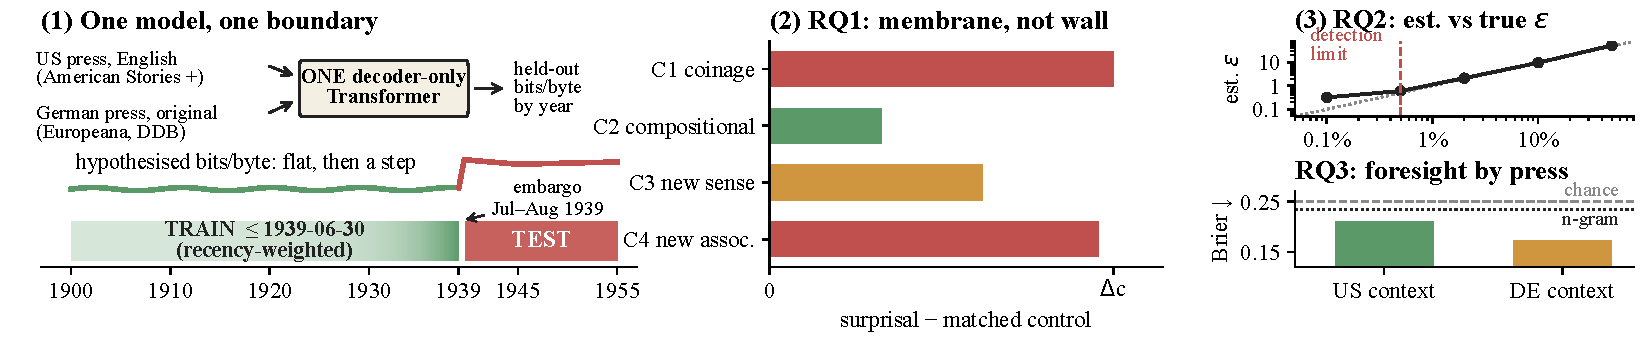
\includegraphics[width=0.97\textwidth]{figures/overview.pdf}
\vspace{-0.7em}
\caption{One model, three measurements. Shapes are hypothesised, not results.}
\end{figure}
\vspace{-1.5em}

\section{Background and Related Work}
Language models degrade on text written after their training window
\citep{lazaridou2021}; temporal conditioning improves calibration on future
facts \citep{dhingra2022}; Time
Machine GPT \citep{drinkall2024} trains point-in-time models uninformed of
later facts. Several recent
projects train models from scratch on historically bounded corpora at cutoffs
across the 19th and early 20th centuries, including 1939
\citep{timecapsule2025,ranke2025,talkie2026}; they aim to \emph{produce} such
models; this project studies the boundary itself. SemEval-2020 Task~1
\citep{schlechtweg2020}, HistBERT \citep{qiu2022} and nineteenth-century models
\citep{hosseini2021} measure how \emph{existing} words drift, using masked
encoders; RQ1 asks which \emph{not-yet-existing} concepts are reachable from a
fixed earlier vocabulary, which needs a causal model with a hard boundary. ChroniclingAmericaQA \citep{piryani2024} shows a large accuracy drop on
uncorrected OCR, motivating OCR quality as a covariate.

\section{Data Processing}
\textbf{Sources, in two stages.} \emph{Corpus~v1} (frozen 10 Oct): American
Stories \citep{dell2023}, article-level (not page-OCR) text from Chronicling America. \emph{Corpus~v2} (frozen 24 Oct) adds non-English
pre-cutoff press translated to English: (i)~foreign-language titles inside
Chronicling America (same metadata and OCR); (ii)~Gallica (FR) and the Deutsches
Zeitungsportal (DE) for the domestic press RQ3 needs --- its $\sim$180 context
articles are translated first, independently of v2; (iii)~Chinese press, as a
stretch. The Transformer trains on v2 if frozen in time, else on v1 with translation
reported as an extension, so no graded result depends on it.
\textbf{Splits} are by publication date, never by shuffling: from every year
1900--1955 a fixed 2\% of articles is held out first and never trained on (the
per-year curve); \textsc{Train}
$=$ the rest $\le$1939-06-30; \textsc{Val} $=$ a disjoint 2\%
$\le$1939-06-30; \textsc{Test-A/B/C} $=$ held-out 1930--38 / 1939-09--1945 /
1946--55. MinHash dedup of wire-service reprints runs \emph{before} splitting. \textbf{Cleaning.}
Per-article OCR quality (period-lexicon hit rate) is a covariate reported by
year and language, with a fixed drop threshold. \textbf{Translation} is data scale, not cleaning: unique pre-1939 tokens bound
how GPT-2-like the model can get, and translation is the only lever that
enlarges them. A fixed-version sentence-level NMT model
(NLLB \citep{nllb2022}; not an LLM, which could add hindsight)
runs on a second machine in parallel, with three defences against its 2020s
English: (1)~any translated sentence containing an RQ1 probe
term is dropped whole; (2)~translated text is never \emph{scored}: it serves as training data and as
RQ3 conditioning context only, and every scored evaluation set is native
English; (3)~its residual probe hit rate is reported, and a held-out translated slice
is scored against native text (the translation-dialect effect). No cap on the translated share; throughput is the bound. \textbf{Tokenizer:} 32k BPE on native-English pre-cutoff text only; all
numbers are bits-per-byte. \textbf{RQ1 probe set:} $\sim$200 post-cutoff terms in four
classes --- C1 coinage (\textit{radar, genocide}), C2 compositional (\textit{atomic
bomb}), C3 old word, new sense (\textit{blitz, resistance}), C4 existing
proper noun, new association (\textit{Pearl Harbor, Hiroshima}) --- each with a frequency-matched
pre-cutoff control in $\ge$5 sentence contexts, frozen in advance. \textbf{RQ2
calibration:} held-out pre-cutoff corpora with a known fraction $\varepsilon$
(0.1--50\%) of 1939-09--1945 articles mixed in. \textbf{RQ3 propositions:} $\sim$60 binary propositions
about 1939--45, each with three same-topic contexts (US, DE, FR press) from June
1939 and from late August 1939 --- the embargo, used as conditioning text only, by explicit exception.

\section{Architecture}
One \textbf{decoder-only Transformer network} as in the Transformer lecture:
token embeddings, stacked blocks of multi-head self-attention and position-wise
feed-forward layers, residual connections, layer normalisation, softmax over the
vocabulary, with attention \textbf{causally masked} (position $i$ sees only
$\le i$) so it is a next-token predictor. Decoder-only is dictated by the
measurements, all sequence probabilities of unseen text: a masked encoder's
pseudo-likelihoods neither form a sequence probability nor score a continuation,
and an encoder--decoder has no source sequence here. This is the GPT-2 configuration. No pretrained weights, and
\textbf{no second Transformer} as control or ablation: all controls are built
at evaluation time on this one model. From scratch in PyTorch, context 1024.
Size
follows data at $\sim$20 tokens/parameter, \textbf{never over two epochs}
(repetition raises memorisation, biasing surprisal): 90M/160M/250M/335M
parameters at $<$1.5B / 1.5--3B / 3--6B / $>$6B tokens; the largest (24 layers,
$d{=}1024$, 16 heads) is $\approx$1.4$\times$10$^{19}$ FLOPs, 30--40\,h on one
RTX~5080, finished before the midterm.
\textbf{Measurement.} For term class $c$, $\Delta_c = \mathbb{E}_{t\in
\mathcal{T}_c}[s(t)] - \mathbb{E}_{t\in\mathcal{C}_c}[s(t)]$, $s$ the model's
surprisal in fixed contexts, $\mathcal{C}_c$ the matched controls. RQ1 is the
profile $(\Delta_{C1..C4})$; RQ2 fits a monotone map to $\varepsilon$ and
reports the minimum detectable $\varepsilon$; RQ3 scores
forced-choice continuations by log-likelihood ratio as Brier score per
perspective; all with bootstrap 95\% CIs.
\textbf{Success:} $\Delta_{C2}$ significantly smallest; a step at 1939, not a
slope; $\hat\varepsilon$ monotone; perspectives above the $n$-gram floor and
significantly different.

\section{Baseline Model}
On the identical training split, tokenizer and token budget, following the
course progression: a \textbf{vanilla RNN}, an \textbf{LSTM} and a
\textbf{GRU} language model, each 2-layer and $\sim$50M parameters, same
next-token objective; the Transformer's choice as primary model is justified by these
comparisons. A \textbf{modified Kneser--Ney 5-gram} (KenLM defaults) is the
non-neural floor; it cannot compose unseen compounds, so it should show no
C1/C2 ordering. All are retrained on the final corpus for reported comparisons.
\textbf{Plan} (individual): baselines 17--24 Oct; the Transformer run 25
Oct--2 Nov; evaluation through November.

\section{Ethical Considerations}
Pre-1939 newspapers carry the racial, ethnic and gender language of their time;
the model will reproduce it, which is documented, not sanitised. Translated
1930s German press includes state propaganda and NMT can misattribute words;
corpus shares by source are reported and RQ3 results are framed as properties
of a record, not verdicts on nations; the RQ2 tool could be misused as an
accusation, so it ships with its detection limit.


\bibliographystyle{plainnat}
\bibliography{references}
\end{document}
